\documentclass{report}
\usepackage{graphicx}
\usepackage{lineno}
\usepackage{ucs}
\usepackage{amsmath}
\usepackage{amsfonts}
\usepackage{listings}
\usepackage[utf8x]{inputenc}
\usepackage[russian]{babel}

\DeclareGraphicsExtensions{.pdf,.png,.jpg}

\newcommand{\ttt}{\hspace*{4mm}}
%\renewcommand{\thesection}{\thechapter.\number\numexpr\value{section}-1\relax}
%\renewcommand{\thesubsection}{\thesection.\number\numexpr\value{subsection}-1\relax}
%\renewcommand{\thesubsubsection}{\thesubsection.\number\numexpr\value{subsubsection}-1\relax}
%\setcounter{secnumdepth}{3}

%\setcounter{chapter}{1}

\begin{document}
\section*{Изменения в приложении}
\ttt
	Для начала я решил превратить свою программу с изображениями в тестовую среду, где можно удобно проверять результаты работы или менять параметры задачи.\\
\ttt
	Для этого я создал 2 окна: 1 с самими графиками, а другое с элементами управления.
		
\center{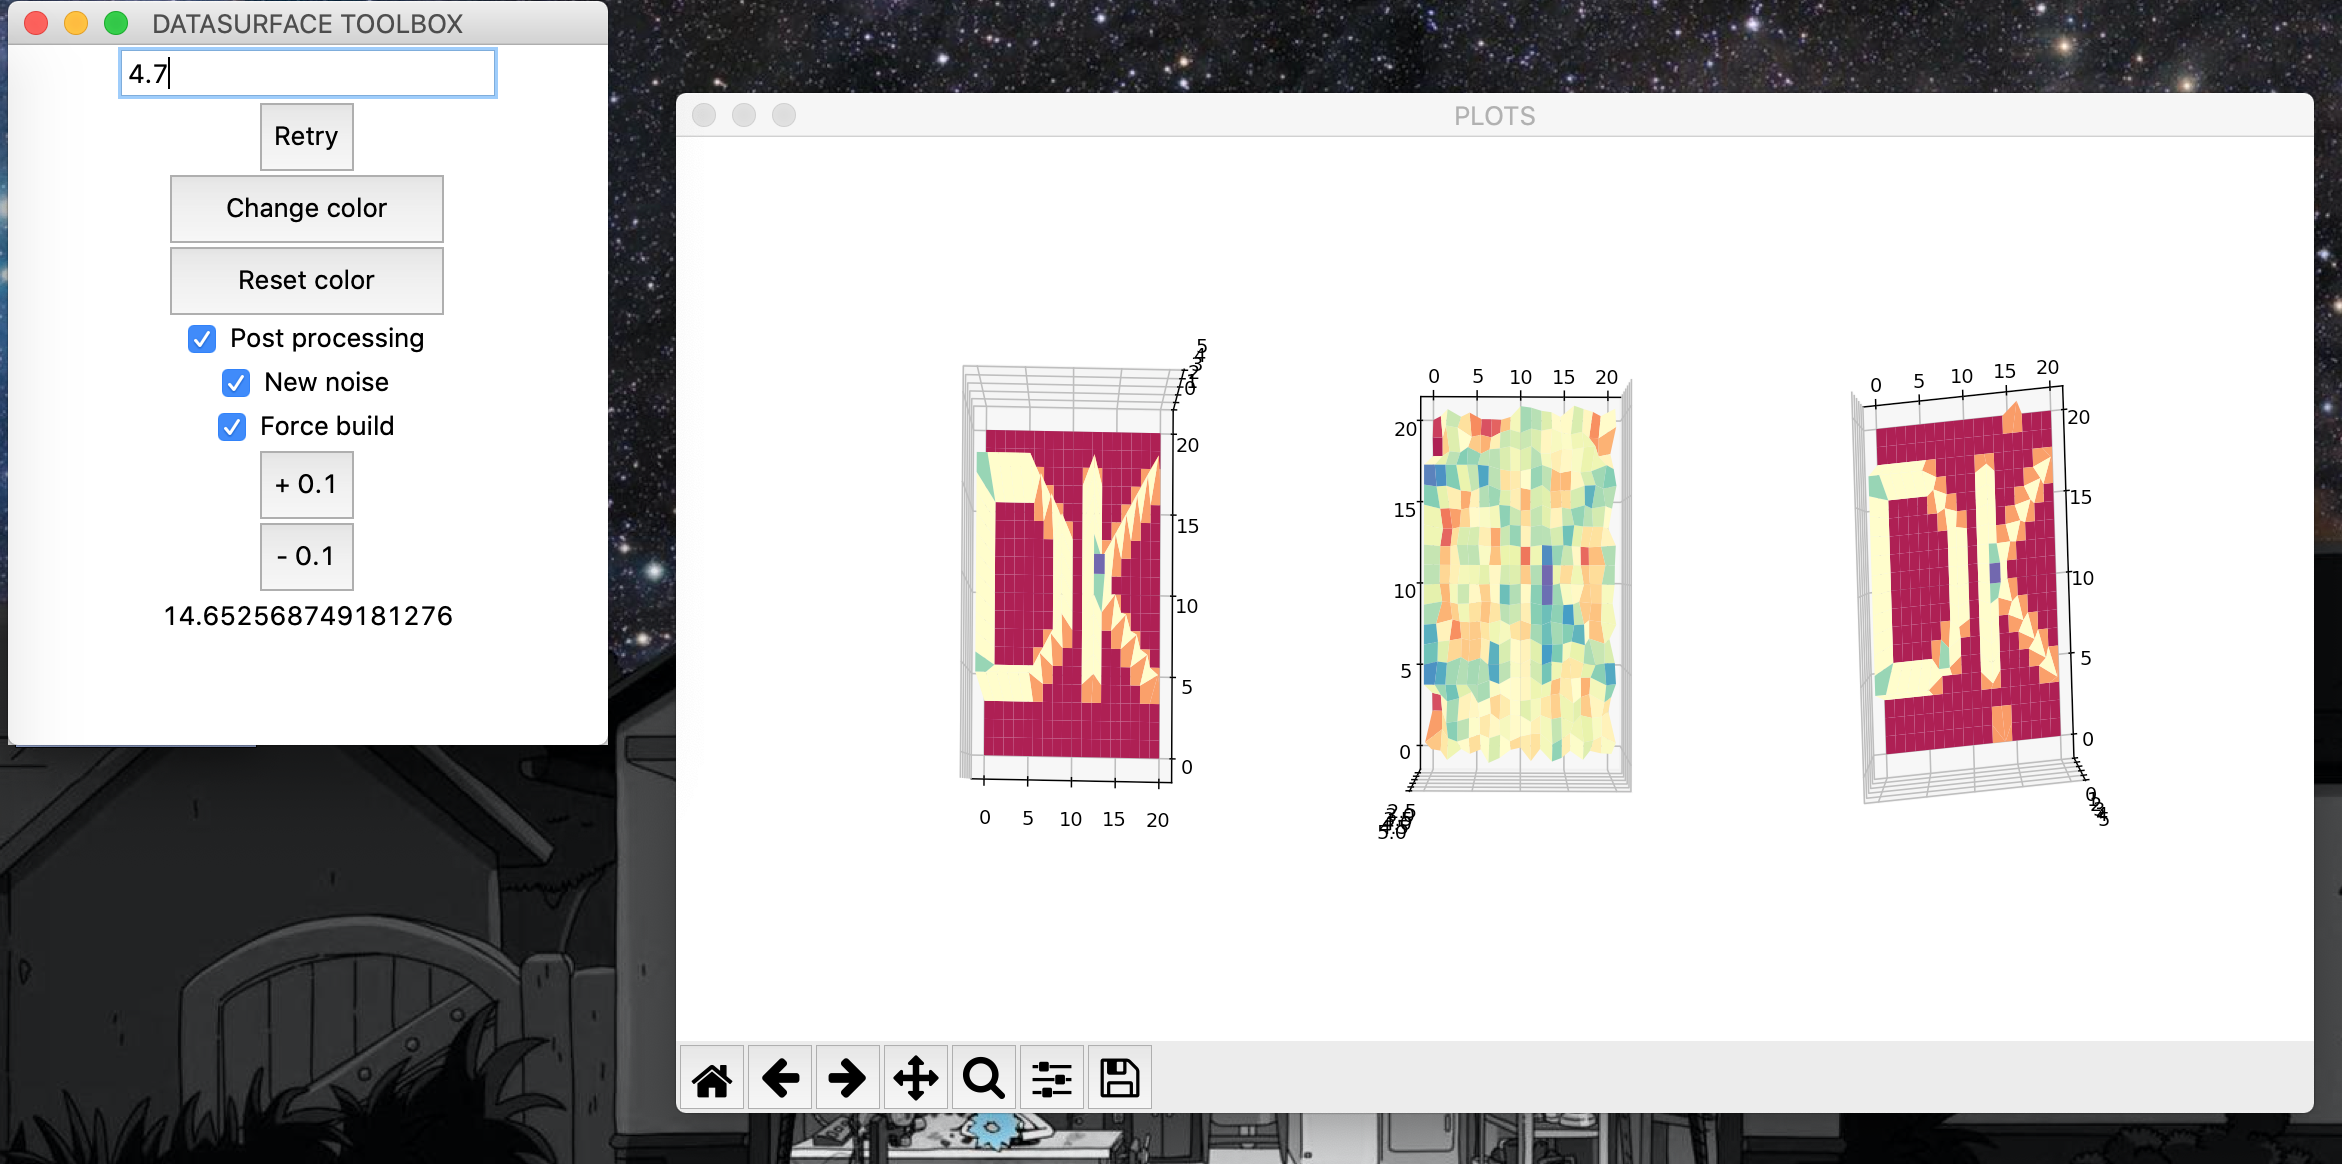
\includegraphics[scale=0.3]{1.png}}
\flushleft
\ttt
Пока что для удобства здесь очень ограниченный функционал, и сделано все средствами питона 3.8 и библиотеки tkinter. Изначально я все сделал в одном окне, но оказалось, что в таком случае ломается разрешение графиков и их очень плохо видно, как будто изображение очень размыто. Я долго искал в гугле решение, но все пишут, что это баг Макинтоша и его экрана Ретина. Возможно есть смысл переписать на C{\lserif\#}, тогда визуально будет более красиво.\\
\bigskip
Перечислю что означают элементы из меню по порядку сверху вниз:
\item 1. Это блок текста, в котором отображается 
значение уровня ошибки, его можно туда вписать руками или нажимать на кнопки и уровнь будет меняться. Соответственно с изменением этого значения графики будут перестраиваться.
\item 2. Кнопка Retry запускает процесс попытки восстановления изображения
\item 3. Change color меняет цвет графиков, т.к. иногда на некоторый тестах плохо различимы отличия в определенном цвете.
\item 4. Reset color возвращает цвет по-умолчанию
\item 5. Post processing нужен для восстановления "интенсивности" \space изображения. Дело в том, что после процесса минимизации функционала восстановленный результат теряет в своих значениях значение самой ошибки. То есть если в определенной точке изначально было значение 5, то в восстановленном изображении c уровнем ошибки 4.7 значение будет 0.3. Post processing добавляет значение ошибки к результату, чтобы он получился близким к идеальному. Но на результатах работы это не отражается и даже без этой функции видно то изображение, которое надо было восстановить.
\item 6. New noise кнопка которая регулирует нужно ли по-новому зашумить изображение при новой попытке или попробовать снова восстановить текущее.
\item 7. Force build нужен для форсирования построения. Иногда процесс минимизации функционала не удается выполнить из-за локальных минимумов или прочих ошибок алгоритма. При включенной кнопке Force build программа будет пробовать восстановить пока ей этого не удастся. При выключенной будет показывать ошибку, из-за чего все пошло не так. Эта функция нужна была мне для отладки. 
\item 8. Далее идут кнопки увеличения/уменьшения уровня ошибки, можно добавить больше вариантов, но легче самому вписывать нужные значения. 
\item 9. И последнее это коэффициент достоверности восстановления. Я сравниваю исходное и восстановленное изображение по точками и вычисляю модуль разности в каждой точке, далее суммирую эти разности и вывожу на экран. Чем меньше этот коэффициент, тем достовернее получилось восстановление. 

\ttt
Во втором окне как и раньше 3 графика слево направо: Исходное изображение, изображение с добавлением шумов, восстановленное изображение. 
\\
\ttt 
Всю программу можно доработать, добавить больше функционала и возможностей. Например, возможность загрузить изображение из файла или может отрисовывать пошагово процесс восстановления для наглядности. Но лучше делать это не средствами питона, а через java script или C{\lserif\#}.
\section*{Что делал.}
\subsection*{1.}
Для начала я переделал способ вычисления интеграла площади 
$$S = \min_{\forall u(x, y) \in U} \iint\limits_\Omega \sqrt{1+(\frac{\partial u}{\partial x})^2 + (\frac{\partial u}{\partial y})^2}dxdy $$
Вычисляю я его по кубатурной формуле Симпсона. 
$$ \iint\limits_\Omega f(x,y)dxdy = \frac{hk}{9} \sum_{i=0}^{2n} \sum_{j=0}^{2m}\lambda_{ij} f_{ij}$$
\newpage

Где $\lambda_{ij}$ являются соответствующими элементами матрицы
\\
$$ \Lambda =
\begin{bmatrix}
1 & 4 & 2 & 4 & 2 & ... & 4 & 2 & 4 & 1\\
4 & 16 & 8 & 16 & 8 & ... & 16 & 8 & 16 & 4\\
2 & 8 & 4 & 8 & 4 & ... & 8 & 4 & 8 & 2\\
... & ... & ... & ... & ... & ... & ... & ... & ... & ...\\
2 & 8 & 4 & 8 & 4 & ... & 8 & 4 & 8 & 2\\
4 & 16 & 8 & 16 & 8 & ... & 16 & 8 & 16 & 4\\
1 & 4 & 2 & 4 & 2 & ... & 4 & 2 & 4 & 1
\end{bmatrix}
$$ 
\\
а $f_{ij}$ - значения функции в точках (i, j).
\\
Реализацию написал самостоятельно. Просто на каждом шаге стою марицу и вычисляю интеграл. 

\subsection*{2.}
Далее моя программа все равно не заработала, и я начал тестировать различные методы численного интегрирования. У меня было \textbf{3} варианта формул, по которым считаются интегралы из 
$$	u = \frac{1}{2}(\int_{x_0}^x q(\xi, y)d\xi + \int_{y_0}^y w(x, \xi)d\xi + u(x, y_0) + u(x_0, y)). $$
\item 1. \textbf{Формула прямоугольников}(правых или левых одинаково) по итогу оказалась самой рабочей. $$ \int_a^b f(x)dx = \sum_{i=0}^{n}f(x_i)(x_{i+1}-x_i). $$
\item 2. \textbf{Формула трапеций}
	$$ \int_a^b f(x)dx = h*(\frac{f(x_0) + f(x_n)}{2})\sum_{i=1}^{n-1}f(x_i). $$

\item 3. \textbf{Формула Симпсона}
$$ \int_a^b f(x)dx = \frac{h}{3}*(f(x_0) + f(x_{2N}) + 2\sum_{j=2,2}^{2N-2}f(x_j) + 4\sum_{j=1,2}^{2N-1}f(x_j)). $$
\\
Для каждого варианта я написал свой вариант программы, что по итогу оказалось трудоемким и немного бесполезным процессом из-за разрывности функции рисунка. Все эти формулы получаются из замены подынтегральной функции интерполяционными многочленами разных степеней, но так как табличные данные -- это поточечно заданная функция, то интерполировать ее у меня не получилось. В картинке нельзя исследовать промежуточное значение функции по известным значениям, так как все значения взяты произвольно.\\
%\newpage
\section*{Ход программы}
\ttt
\textit{В этом разделе описаны шаги восстановления изображения, описанные в приложении.} \\
\subsection*{Заполнение тестовых данных}
\ttt Для начала я заполняю исходную матрицу так, чтобы получался рисунок. В матрицу [20х20] в нужные точки кладу значение lVal, а в пустых узлах оставляю 0. \\
\center{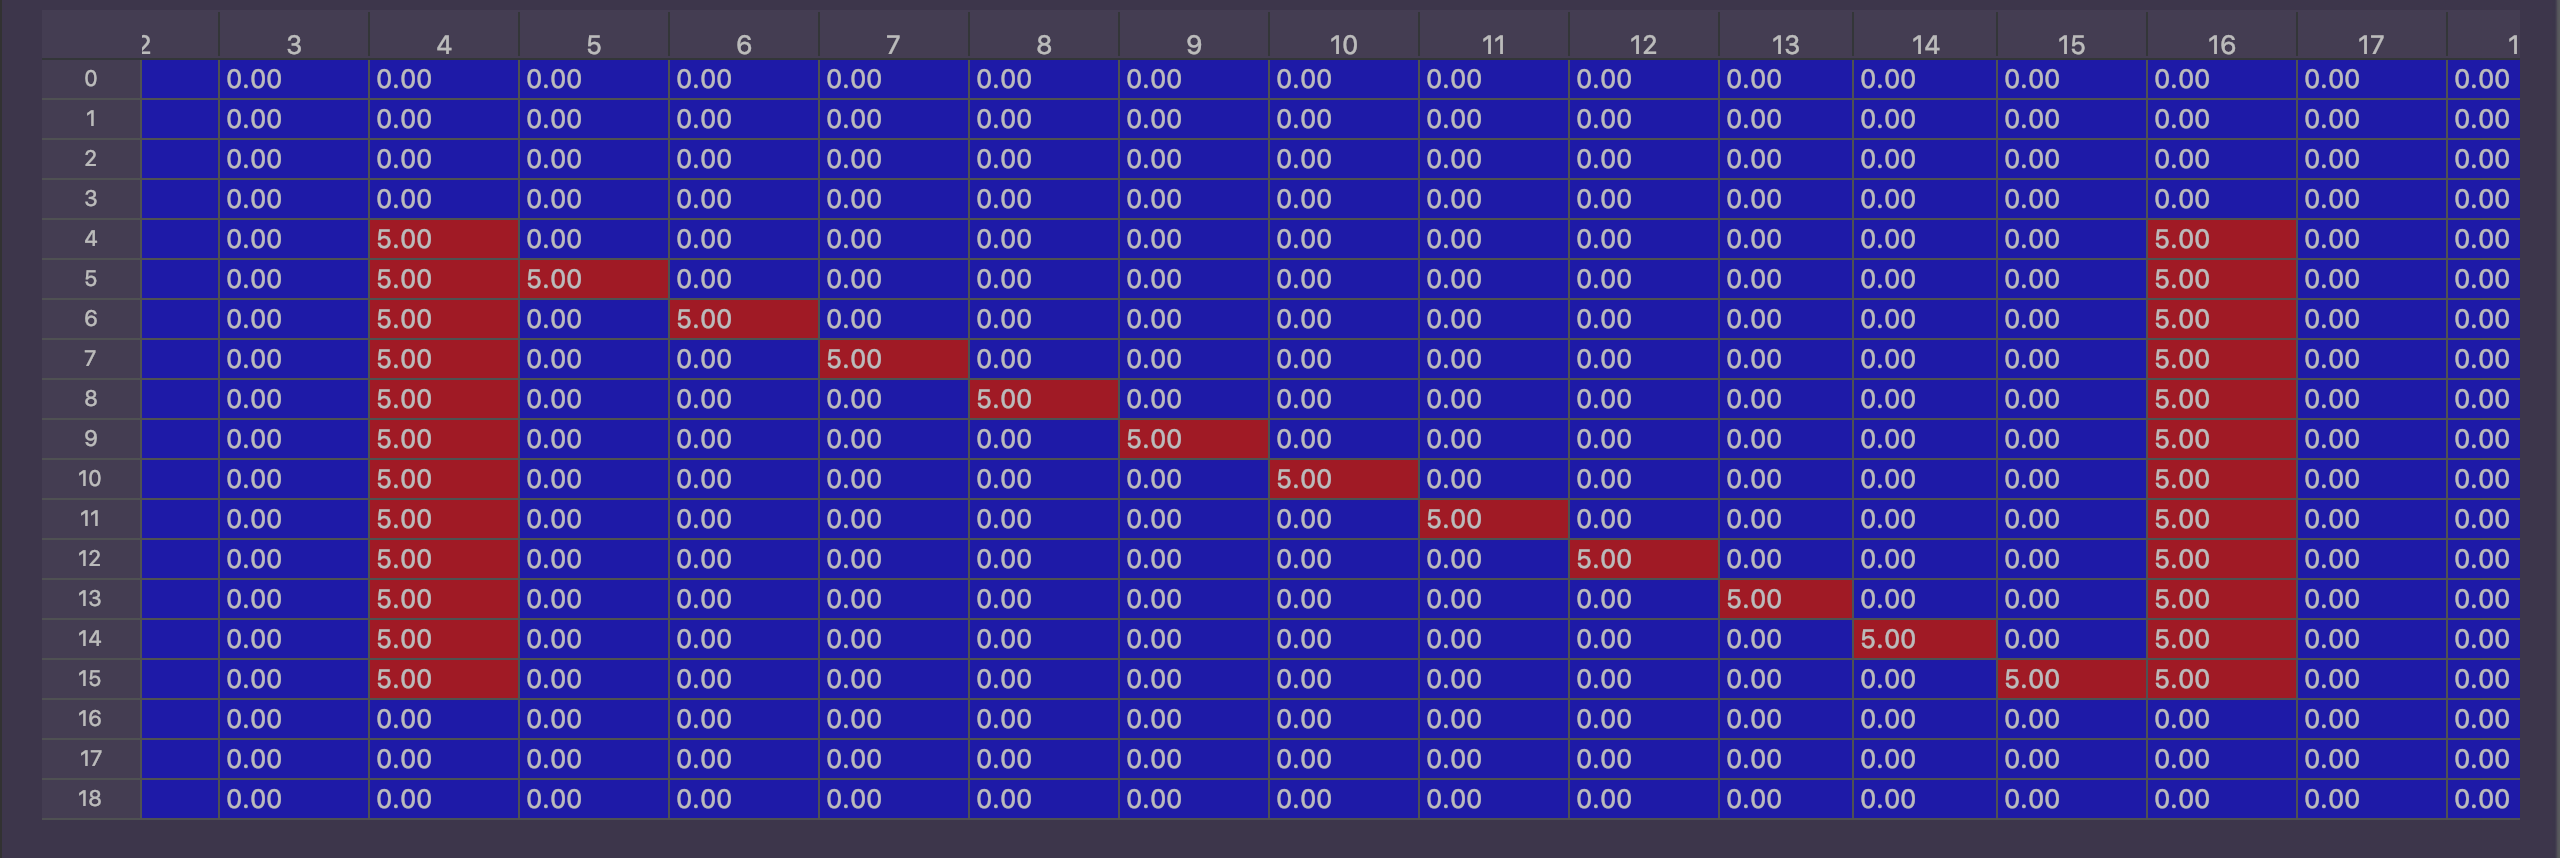
\includegraphics[scale=0.3]{2.png}}
Пример для буквы N и lVal = 5
\flushleft
Далее идет добавление шумов к картинке. Используя генератор рандомных чисел, я к каждой точке добавляю случайное вещественное число $\leq lVal$. Если шумы больше, чем "интенсивность"\space самого рисунка, то возникает неопределенность при минимизации, и такой рисунок не удается однозначно восстановить. 
\center{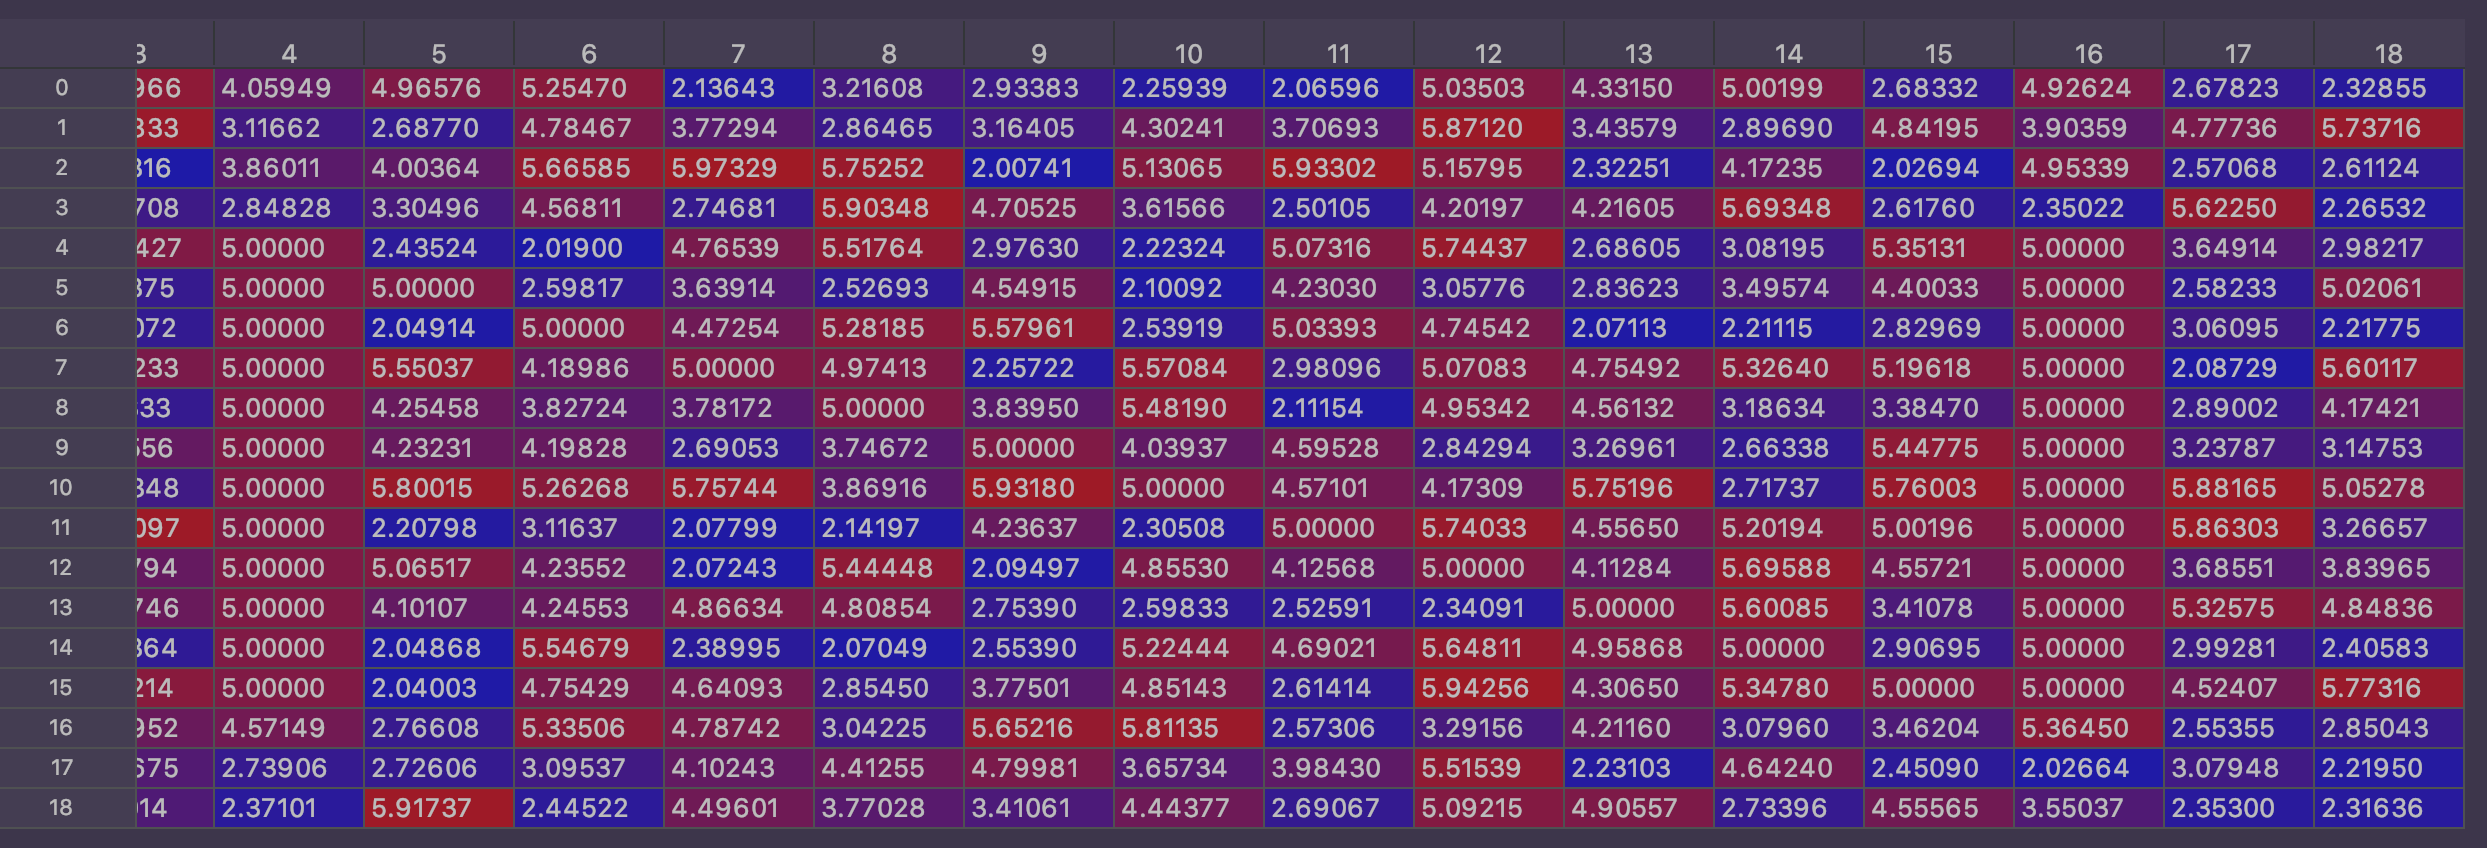
\includegraphics[scale=0.3]{3}}
Зашумленная матрица
\clearpage
Вот так выглядят исходная и зашумленная матрицы с буквой
\\
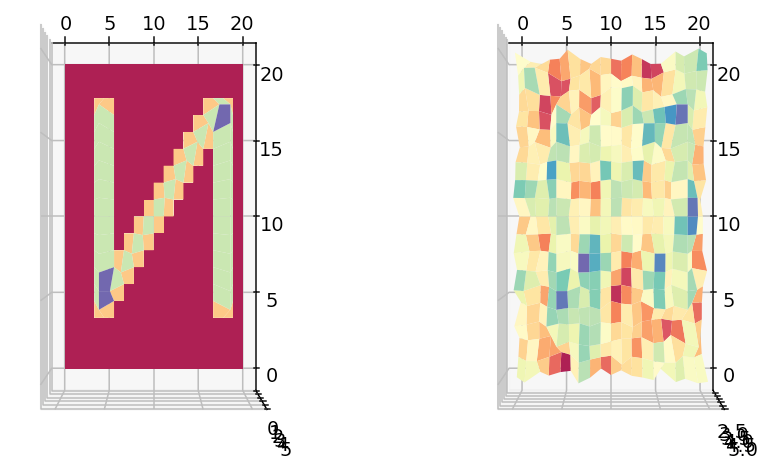
\includegraphics[scale=0.6]{4.png}
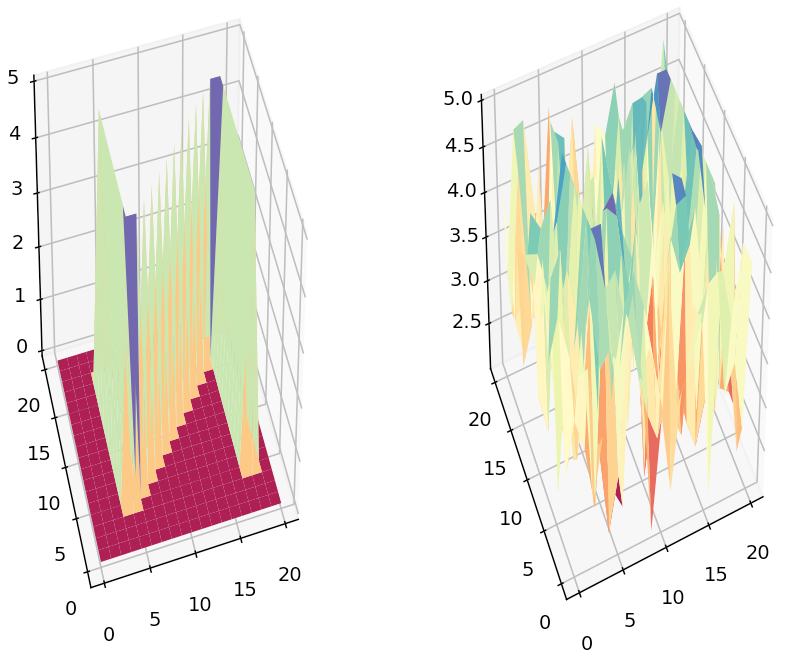
\includegraphics[scale=0.5]{5.png}
\\\flushleft
\subsection*{Восстановление изображения}
\ttt Далее начинается процесс восстановления. Пусть
$ u_{ij} = u(x_i,y_j);$
\\
В формуле для $u_{ij} = \frac{1}{2}(\int_{x_0}^{x_i} q(\xi, y)d\xi + \int_{y_0}^{y_j} w(x, \xi)d\xi + u_{i0} + u_{oj})$ используются значения $u_{i0}$ и $u_{oj}$. Поэтому сначала вычисляются граничные значения $u_{i0}$ и $u_{oj}$  $\forall i \in 1, 2, ...,N$ $\forall j \in 1, 2, ...,N$ по формулам:
$$ u_{i0} = \frac{1}{2}(\int_{x_0}^{x_i} q(\xi, y)d\xi + u_{00} + u_{i0}) = \int_{x_0}^{x_i} q(\xi, y)d\xi + u_{00}$$
$$ u_{0j} = \frac{1}{2}(\int_{y_0}^{y_i} w(x, \xi)d\xi + u_{00} + u_{0j}) = \int_{y_0}^{y_i} w(x, \xi)d\xi + u_{00}$$
Соответственно для каждого из 3 вариантов я запрограммировал следующие формулы:
\item 1. \textbf{Прямоугольники}
	$$ u_{i0} = \sum_{k=0}^{i}q_{k0} + u_{00};\ttt u_{0j} = \sum_{k=0}^{j}w_{0k} + u_{00};$$
\item 2. \textbf{Трапеции}
	$$ u_{i0} = \frac{q_{00} + q_{i0}}{2} + \sum_{k=1}^{i-1}q_{k0} + u_{00};\ttt u_{0j} = \frac{w_{00} + w_{0j}}{2} +  \sum_{k=1}^{j-1}w_{0k} + u_{00};$$
\item 3. \textbf{Симпсон}
	$$ u_{i0} = \frac{1}{3} (q_{00} + q_{i0} + 2\sum_{k=2,2}^{i-1}q_{k0} + 4\sum_{k=1,2}^{i-1}q_{k0} )+ u_{00};\ttt u_{0j} = \frac{1}{3} (w_{00} + w_{0j} + 2\sum_{k=2,2}^{j-1}w_{0k} + 4\sum_{k=1,2}^{j-1}w_{0k} )+ u_{00};$$
\\
\ttt Минимизация функционала площади выполняется по переменным $q = \frac{\partial u}{\partial x}$ и $w = \frac{\partial u}{\partial y}$. В начале работы алгоритма заполняются ограничивающие неравенства $|u_{ij} - a_{ij}| \leq \sigma$ относительно искомых $q_{i0}$ и $w_{0j}$. Далее минимизируются функционал  $\int\sqrt{1+r^2(x)}dx$. Получаем искомые минимальные $q_{i0}$ и $w_{0j}$ и вычисляются $u_{i0}$ и $u_{0j}$\\
\ttt После вычисления всех граничных значений происходит вычисление во внутренних узлах сетки.
\item 1. \textbf{Прямоугольники}
	$$ u_{ij} = \frac{1}{2}( \sum_{k=0}^{i}q_{kj} + \sum_{k=0}^{j}w_{ik} + u_{i0} + u_{0j});$$
\item 2. \textbf{Трапеции}
	$$ u_{ij} = \frac{1}{2}(\frac{q_{0j} + q_{ij}}{2} +\sum_{k=1}^{i-1}q_{kj} + \frac{w_{0i} + w_{ij}}{2}+\sum_{k=1}^{j-1}w_{ik} + u_{i0} + u_{0j});$$
\item 3. \textbf{Симпсон}
	$$ u_{ij} = \frac{1}{2}(\frac{1}{3} (q_{0j} + q_{ij} + 2\sum_{k=2,2}^{i-1}q_{kj} + 4\sum_{k=1,2}^{i-1}q_{kj} ) + \frac{1}{3} (w_{i0} + w_{ij} + 2\sum_{k=2,2}^{j-1}w_{ik} + 4\sum_{k=1,2}^{j-1}w_{ik} )+ u_{i0}+ u_{0j});$$
\\
\ttt Аналогично граничному случаю, сначала заполняются ограничивающие неравенства $|u_{ij} - a_{ij}| \leq \sigma$, затем минимизация исходного функционала площади $\iint\limits_\Omega \sqrt{1+(q)^2 + (w)^2}dxdy$. Получаем искомые минимальные $q_{ij}$ и $w_{ij}$. Подставив их обратно в формулу для $u_{ij}$, вычисляется сам $u_{ij}$ и т.д.\\
\ttt Таким образом получается пошагово восстановленная матрица и она выводится на экран 3 графиком. В данный момент я использую 1 уровень ошибки на всех узлах сетки.\\
\ttt Также я ввел погрешность минимизации. Иногда в результате минимизации вместо 0 получаются невероятно маленькие, но положительные значения. Погрешность минимизации нужна, чтобы в таких случаях считать значения 0, т.к. иначе эти маленькие значения накапливаются и входят в сумму при численном интегрировании, что уменьшает точность результата. 
\section*{Итоги и тесты}

\end{document} 